\section{Availability}\label{sec:availability}

%Internet connectivity in developed countries could be considered an ``always
%on'' resource. In this section we look at the availability of Internet
%connectivity. 

We first study the extent to which Internet connectivity was available across
the home broadband networks in our deployment, and whether any remarkable
availability or usage patterns emerged.  We observe the frequency and duration
of downtime across the deployment and the extent to which these characteristics
differ between home networks---we explore differences between
\developing{} and \developed{} countries (and specifically, how downtime
characteristics vary according to a country's GDP), as well as usage
patterns that are unique to individual homes.

We measure the availability of
Internet connectivity by recording periodic heartbeat messages
which every router sends to our central server approximately once per minute. The
arrival of a heartbeat signifies that the router is up and connected to
the Internet.  We define {\em downtime} as any gap in the heartbeat
logs that lasts longer than ten minutes.  The absence of a heartbeat
could signify that the router is offline, has been shut down or
rebooted, or that the heartbeat was lost.  For reboots the
router usually comes back up within a few minutes. In some cases, we can
positively verify downtimes caused by powered off routers using the Uptime data set. All results in
this section are based on the Heartbeats and Uptime data sets, as described in
Section~\ref{sec:data}.  Table~\ref{tab:availability-results} summarizes
a few of the more interesting results.


\begin{table}[t]
\begin{small}
\begin{tabular}{|p{2.6in}l|}
\hline
& \\

Developed countries experience far less frequent extended downtime than
\developing{} countries: The median time between downtime in \developed{}
countries is more than a month while in \developing{} countries it is
less than a day. & \S\ref{sec:uptime}, Fig.~\ref{fig:cdf-outages} \\ & \\
%
The two countries in our deployment with the most frequent downtime are those with
the lowest per-capita GDP (India and Pakistan). & \S\ref{sec:uptime},
Fig.~\ref{fig:outages-scatter} \\ & \\
%
In some cases in \developing{} countries, broadband connectivity is not
``always on'' because users only turn on their routers to use the
Internet. & \S\ref{sec:avail-case}, Fig.~\ref{fig:china-availability} \\ & \\
\hline
\end{tabular}
\end{small}
\caption{Highlights of Section~\ref{sec:availability} results.}
\label{tab:availability-results}
\end{table}


\subsection{How reliable is home broadband access?}\label{sec:uptime}

We study the ``uptime'' of home broadband Internet access across home
networks in our deployment, in terms of the frequency and duration of
downtime.  We also explore the extent to which these characteristics vary
by country.

\begin{figure}[t]
  \begin{minipage}{\linewidth}
  \includegraphics[width=0.98\linewidth]{figures/cdf_avg_downtimes_per_day_clean}
  %\includegraphics[width=0.98\linewidth]{figures/cdf_avg_outages_per_day_v2}
%  \subfloat[For \groupa{}, 20\% of users see an outage more than once every 10 days]{
%  \includegraphics[width=0.98\linewidth]{figures/cdf_outage_num_rc}
%  \label{fig:cdf-outage-developed}}\\
%  \subfloat[For \groupb{}, about 50\% of users see an outage every 3 days]{
%  \includegraphics[width=0.98\linewidth]{figures/cdf_outage_num_nsrc}
%  \label{fig:cdf-outage-developing}}
  \end{minipage}
  \caption{Average number of downtimes per day that last at least ten
    minutes. Developed countries experience far fewer downtimes per day than 
developing countries.}
  \label{fig:cdf-outages}
\end{figure}


\begin{figure}[t]
  \begin{minipage}{\linewidth}
  \includegraphics[width=0.98\linewidth]{figures/cdf_downtime_duration_clean}
  %\includegraphics[width=0.98\linewidth]{figures/cdf_median_outage_duration_clean}
  %\includegraphics[width=0.98\linewidth]{figures/cdf_outage_duration}
  \caption{Downtime duration for developing and developed
    countries. The median downtime duration 
   is similar, but as we see in Figure~\ref{fig:cdf-outages}, 
   developing countries see downtime much more frequently.}
  \label{fig:cdf-outage-duration}
  \end{minipage}
\end{figure}


\begin{figure}[t]
  \begin{minipage}{\linewidth}
  \includegraphics[width=0.98\linewidth]{figures/num_downtimes_scatter_clean_v2}
  %\includegraphics[width=0.98\linewidth]{figures/num_outages_scatter_clean}
  %\includegraphics[width=0.98\linewidth]{figures/outages_scatter_april}
  \caption{The median number of downtimes across homes in each
    country during October 2012 -- April 2013 vs. the GDP of the country where that home
    network was located. The marker size is proportional to the median downtime duration
    in that country. The vertical line separates
    developing and developed countries. We show only countries with
    at least three routers deployed.}
  \label{fig:outages-scatter}
  \end{minipage}
\end{figure}



\paragraph{Frequency of downtime.}  Figure~\ref{fig:cdf-outages} shows a
distribution of the downtime over six months, for both \developed{} and
\developing{} countries; we show a distribution of the average number of
downtimes per day for each network, where downtime is defined as an interruption
in connectivity of ten minutes or longer.  As expected, the home networks in
\developing{} countries sustain substantially more downtime compared to those in
\developed{} countries. The median duration between downtimes for networks in
\developed{} countries is more than a month, whereas for \developing{}
countries, the median duration between downtimes is less than a single day.

\paragraph{Duration of downtime.}
Figure~\ref{fig:cdf-outage-duration} shows a cumulative distribution function
of the downtime durations for both \developing{} and
\developed{} countries.  The plot shows that the median downtime duration 
is approximately 30 minutes, and that downtime in \developing{}
countries tend to last longer.  Downtime sometimes lasts several days.  

\paragraph{Downtime characteristics vs. per-capita GDP.}
Figure~\ref{fig:outages-scatter} shows a scatter plot of the median
number of downtimes experienced by home networks in each country vs. the
{\em per-capita GDP} for that country in U.S. dollar equivalent (\ie,
the purchasing power parity)~\cite{www-imf-gdp} for countries with at
least three deployed routers.  The vertical line divides
nine \developing{} from eleven \developed{} countries.  Although
there is no discernible difference between any of the \developing{} and
\developed{} countries in terms of the median number of downtimes, the two
countries with the lowest per-capita GDP in our deployment---India and
Pakistan---experienced significantly more downtime during October 1, 2012 -- April 15,
2013. A home network in Pakistan experienced nearly two downtimes lasting
at least ten minutes every day.\footnote{These characteristics are are
  based on data from about 12 routers in India and about five routers in
  Pakistan for October 1, 2012 -- April 15, 2013.  In general, some country data from
  this scatter plot may be inconclusive, due to the small number of
  countries from which we collect data, but the trend appears to hold
  for at least the poorest countries.}


\subsection{Case Study: Router as Home Appliance}\label{sec:avail-case}

\begin{figure}[t]
    \begin{minipage}{\linewidth}
    \subfloat[This household never intentionally turns off its router,
    which is typical of routers in developed countries.]{
        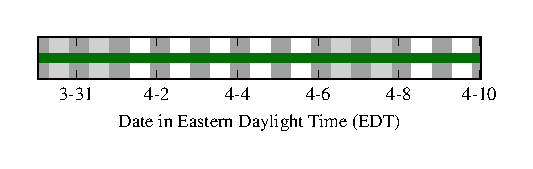
\includegraphics{figures/developed_availability}
        \label{fig:developed-availability}
    }

    \subfloat[This household often turns off its router when not using it. The
    router is available briefly in evenings and during weekends.]{
        
\includegraphics{figures/china_availability}
        \label{fig:china-availability}
    }

    \subfloat[This household's access link experienced sporadic ISP outages for
    several days in April 2013. Although the router was continuously powered on,
we label this as downtime.]{
        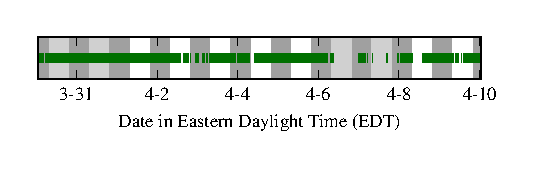
\includegraphics{figures/comcast_availability}
        \label{fig:comcast-availability}
    }
    \caption{Examples of different modes of router availability. The thick
        horizontal green lines indicate intervals when the router is {\em
        available}. For reference, dark shaded regions indicate nighttime hours and
        lighter shaded regions indicate weekend daylight hours.}
    \end{minipage}
\end{figure}


In addition to general trends, we also discovered some interesting cases of
availability and usage patterns.  We observed that in the United States, most
users leave their routers powered on all of the time.
The median US user has his router on 98.25\% of time in the measured time period.
Router availability in these homes resembles Figure 6a.
In contrast, 
{\em home broadband is not ``always on'' in the developing world.}
As a comparison, median routers in India and South Africa stay on only for 76.01\% and 
85.57\% of the time, respectively.  
We observed cases where users powered their router on for specific
time periods when they were using the Internet, much as someone would use any
other appliance. 
We envision multiple
possible reasons for this disparity. One reason could be {\em behavioral patterns}: in some
cases, we can observe specific patterns where users power down their
router when they are not actively using it (because of data usage caps
imposed by certain ISPs).  For example,
Figure~\ref{fig:china-availability} shows one Chinese household that
consistently keeps its router off except during the early
evening. During the weekend, the router is on for longer periods,
presumably with increased activity.  
Another reason could be {\em poor
  connectivity}, such as high loss or network outages caused by
congestion, overload, or even poor infrastructure or
equipment, as is possibly the case for the home network in
Figure~\ref{fig:comcast-availability}.
